% ------------------------------------------------------------------------------
% Slide 9: Por Qué se Perdió la Separación: Ritmo, Pantalla y Cámara
% ------------------------------------------------------------------------------
\begin{frame}{Por Qué se Perdió la Separación: Ritmo, Pantalla y Cámara}
    \begin{columns}[c]
        \begin{column}{0.51\textwidth}
            \scriptsize
            \begin{block}{Hipótesis que Probamos Estas Semanas}
                \begin{itemize}\setlength{\itemsep}{1pt}\setlength{\parskip}{0pt}
                    \item \textbf{Anticiparse al metrónomo:} Quisimos evitar que la persona entre en automático agregando un atraso variable ($\Delta t$). Si el cambio de tiempo es muy rápido, se pierde todavía más el patrón (falta ajustar bien el rango de $\Delta t$).
                    \item \textbf{Mirar las ondas en la pantalla:} Ver la señal en vivo hacía que el usuario cambie la fuerza o corrija sobre la marcha. En los nuevos ensayos se usa \textbf{pantalla limpia} mostrando solo la letra a pronunciar.
                \end{itemize}
            \end{block}
            \vspace{0.03cm}
            \begin{alertblock}{La Cámara como Control del Experimento}
                \begin{itemize}\setlength{\itemsep}{1pt}\setlength{\parskip}{0pt}
                    \item \textbf{Uso exclusivo de control:} La cámara de video se usa únicamente para verificar el movimiento de la cara, nunca como parte del decodificador final (que es 100\% EMG).
                    \item \textbf{Prueba clave:} Si los puntos de la cara en la cámara tampoco separan las vocales en un PCA, confirmamos que la diferencia no está en el rostro sino adentro, en la lengua.
                \end{itemize}
            \end{alertblock}
        \end{column}
        \begin{column}{0.47\textwidth}
            \centering
            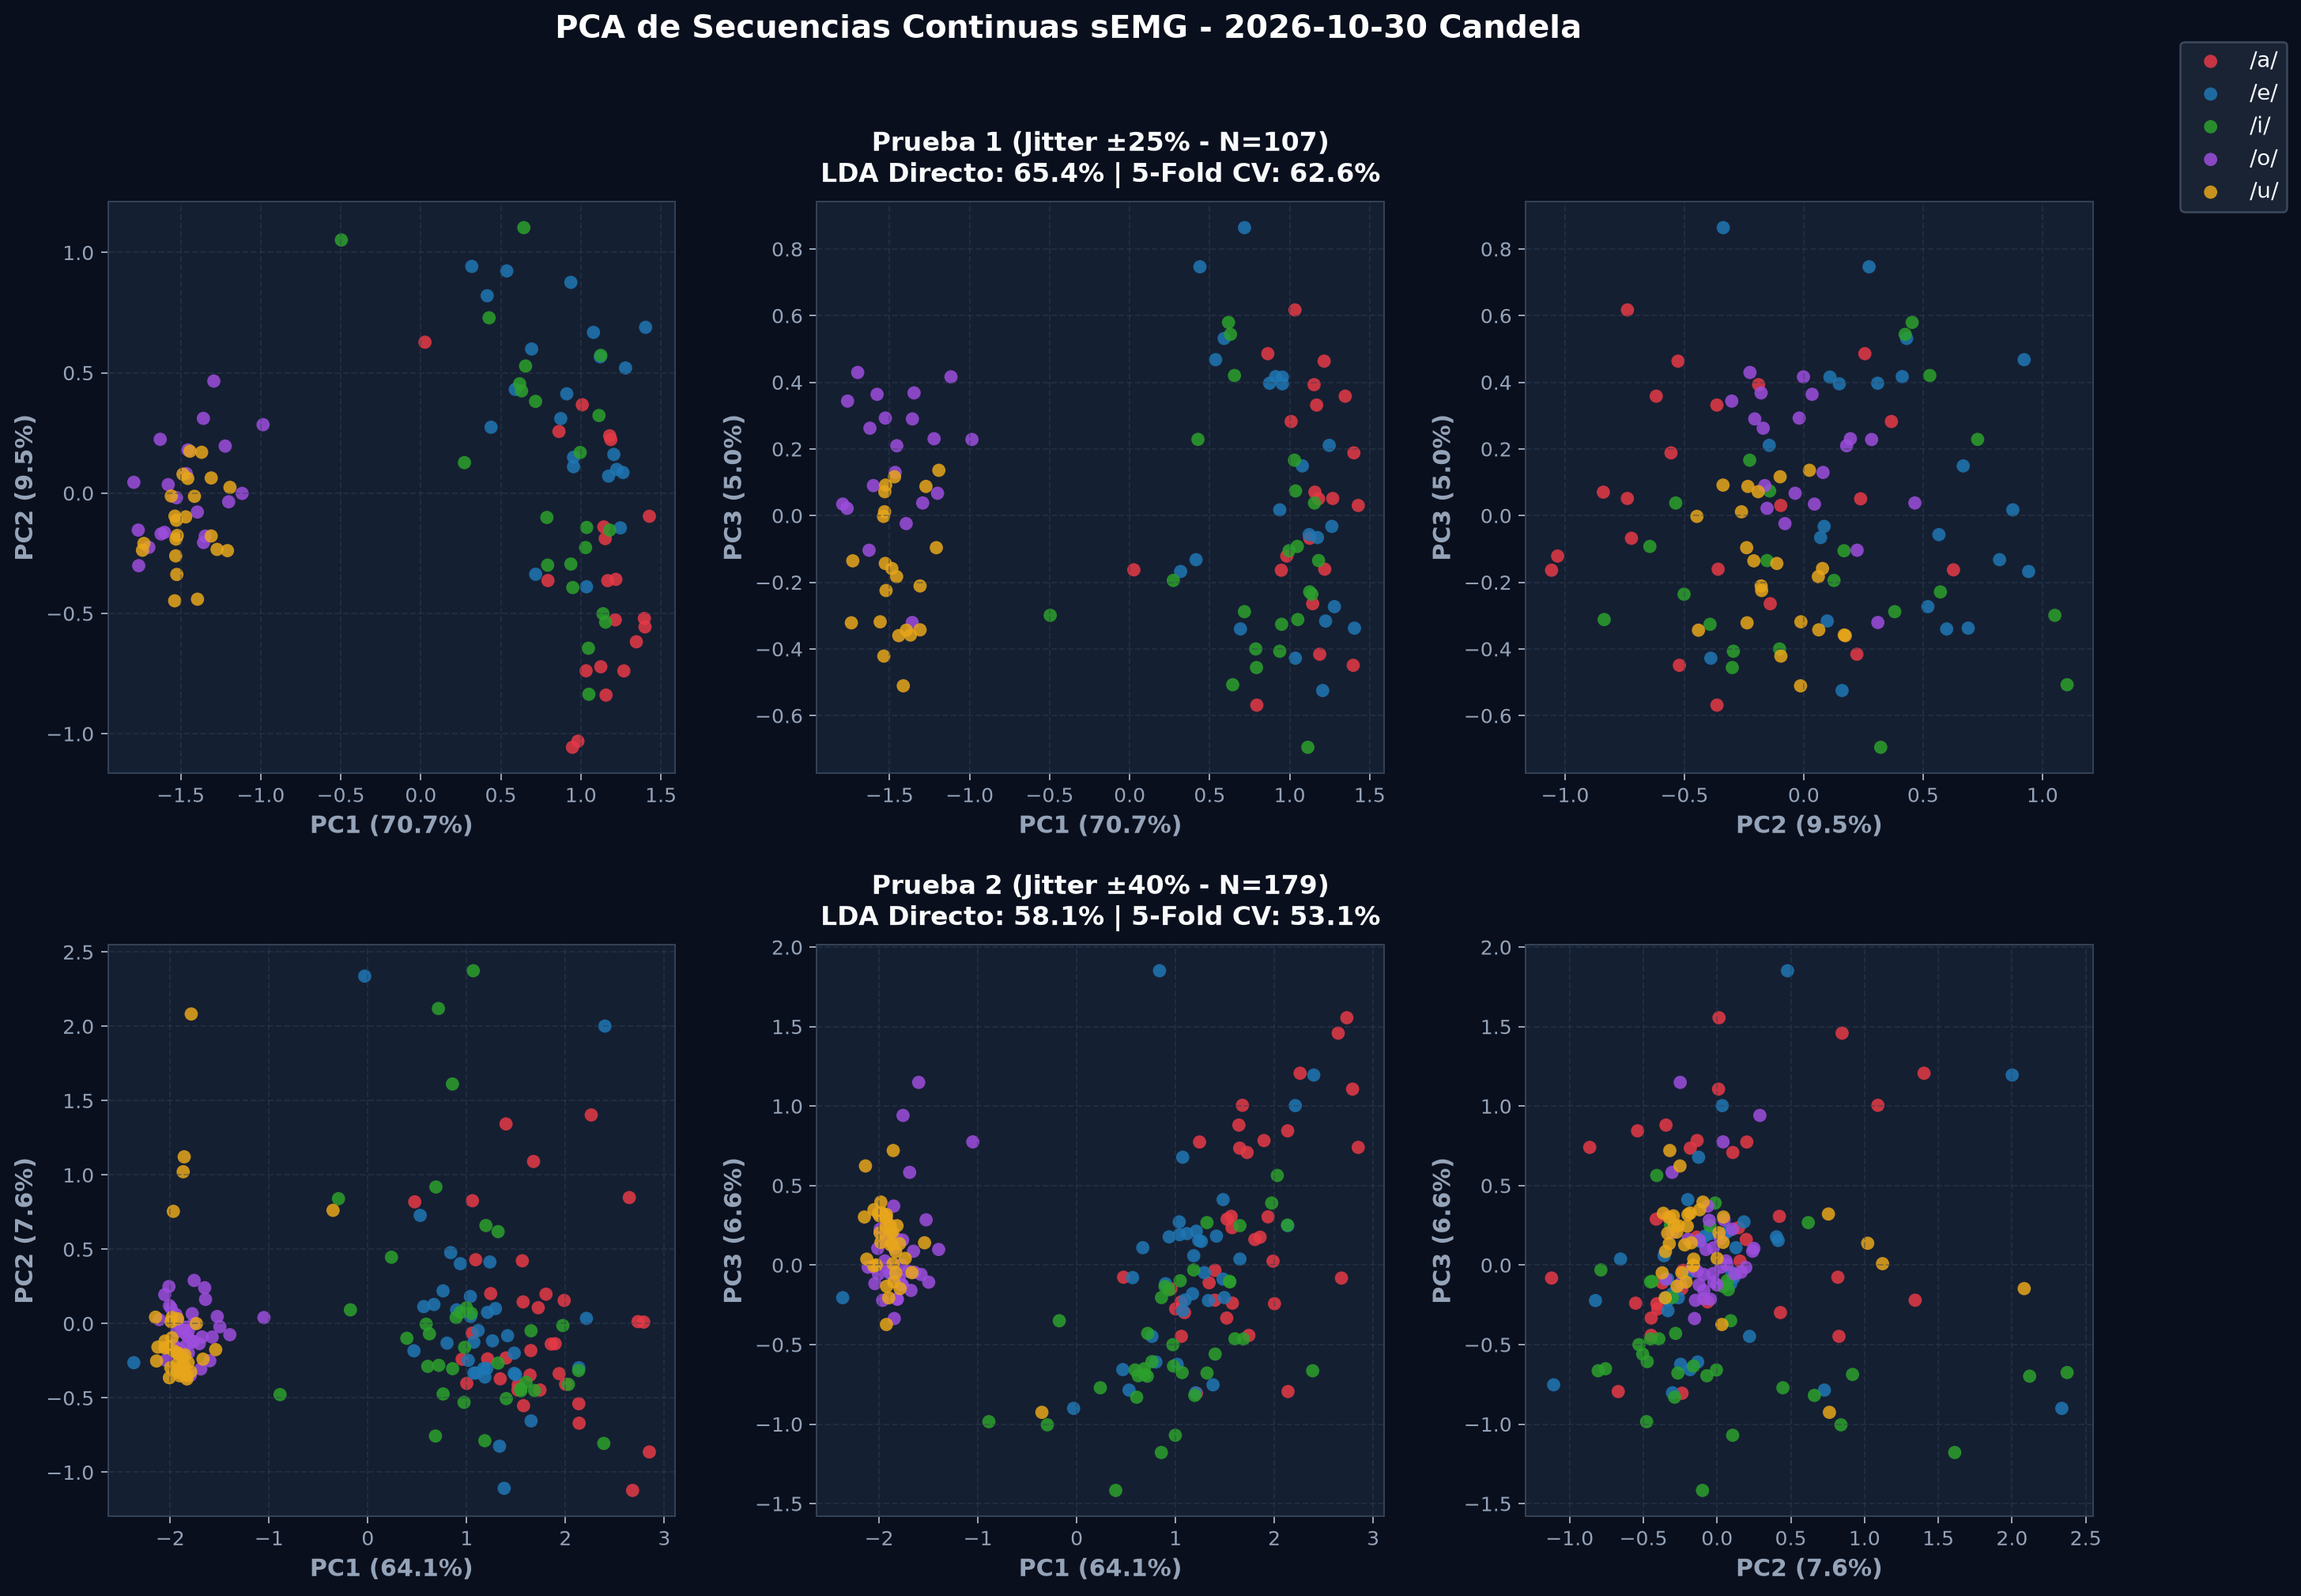
\includegraphics[width=\linewidth,height=0.72\textheight,keepaspectratio]{figuras/pca_comparativo_secuencias_continuas_jittering.png}
        \end{column}
    \end{columns}
\end{frame}
